%  LaTeX support: latex@mdpi.com 
%  For support, please attach all files needed for compiling as well as the log file, and specify your operating system, LaTeX version, and LaTeX editor.

%=================================================================
\documentclass[entropy,article,submit,pdftex,moreauthors]{Definitions/mdpi} 
% For posting an early version of this manuscript as a preprint, you may use "preprints" as the journal and change "submit" to "accept". The document class line would be, e.g., \documentclass[preprints,article,accept,moreauthors,pdftex]{mdpi}. This is especially recommended for submission to arXiv, where line numbers should be removed before posting. For preprints.org, the editorial staff will make this change immediately prior to posting.

%--------------------
% Class Options:
%--------------------
%----------
% journal
%----------
% Choose between the following MDPI journals:

%---------
% article
%---------
% The default type of manuscript is "article", but can be replaced by: 
% abstract, addendum, article, book, bookreview, briefreport, casereport, comment, commentary, communication, conferenceproceedings, correction, conferencereport, entry, expressionofconcern, extendedabstract, datadescriptor, editorial, essay, erratum, hypothesis, interestingimage, obituary, opinion, projectreport, reply, retraction, review, perspective, protocol, shortnote, studyprotocol, systematicreview, supfile, technicalnote, viewpoint, guidelines, registeredreport, tutorial
% supfile = supplementary materials

%----------
% submit
%----------
% The class option "submit" will be changed to "accept" by the Editorial Office when the paper is accepted. This will only make changes to the frontpage (e.g., the logo of the journal will get visible), the headings, and the copyright information. Also, line numbering will be removed. Journal info and pagination for accepted papers will also be assigned by the Editorial Office.

%------------------
% moreauthors
%------------------
% If there is only one author the class option oneauthor should be used. Otherwise use the class option moreauthors.

%---------
% pdftex
%---------
% The option pdftex is for use with pdfLaTeX. If eps figures are used, remove the option pdftex and use LaTeX and dvi2pdf.

%=================================================================
% MDPI internal commands
\firstpage{1} 
\makeatletter 
\setcounter{page}{\@firstpage} 
\makeatother
\pubvolume{1}
\issuenum{1}
\articlenumber{0}
\pubyear{2022}
\copyrightyear{2022}
%\externaleditor{Academic Editor: Firstname Lastname}
\datereceived{} 
%\daterevised{} % Only for the journal Acoustics
\dateaccepted{} 
\datepublished{} 
%\datecorrected{} % Corrected papers include a "Corrected: XXX" date in the original paper.
%\dateretracted{} % Corrected papers include a "Retracted: XXX" date in the original paper.
\hreflink{https://doi.org/} % If needed use \linebreak
%\doinum{}
%------------------------------------------------------------------
% The following line should be uncommented if the LaTeX file is uploaded to arXiv.org
%\pdfoutput=1

%=================================================================
% Add packages and commands here. The following packages are loaded in our class file: fontenc, inputenc, calc, indentfirst, fancyhdr, graphicx, epstopdf, lastpage, ifthen, lineno, float, amsmath, setspace, enumitem, mathpazo, booktabs, titlesec, etoolbox, tabto, xcolor, soul, multirow, microtype, tikz, totcount, changepage, attrib, upgreek, cleveref, amsthm, hyphenat, natbib, hyperref, footmisc, url, geometry, newfloat, caption

%=================================================================
%% Please use the following mathematics environments: Theorem, Lemma, Corollary, Proposition, Characterization, Property, Problem, Example, ExamplesandDefinitions, Hypothesis, Remark, Definition, Notation, Assumption
%% For proofs, please use the proof environment (the amsthm package is loaded by the MDPI class).

%=================================================================
% Full title of the paper (Capitalized)
\Title{On the Universally Optimal Activation Function for a Class of Residual Neural Networks}

% MDPI internal command: Title for citation in the left column
\TitleCitation{Title}

% Author Orchid ID: enter ID or remove command
\newcommand{\orcidauthorA}{0000-0002-5300-668X} % Add \orcidA{} behind the author's name
%\newcommand{\orcidauthorB}{0000-0000-0000-000X} % Add \orcidB{} behind the author's name

% Authors, for the paper (add full first names)
\Author{Feng Zhao $^{1,\dagger,\ddagger}$\orcidA{}, Shao-Lun Huang $^{2,\ddagger}$*}

%\longauthorlist{yes}

% MDPI internal command: Authors, for metadata in PDF
\AuthorNames{Firstname Lastname, Firstname Lastname and Firstname Lastname}

% MDPI internal command: Authors, for citation in the left column
\AuthorCitation{Lastname, F.; Lastname, F.; Lastname, F.}
% If this is a Chicago style journal: Lastname, Firstname, Firstname Lastname, and Firstname Lastname.

% Affiliations / Addresses (Add [1] after \address if there is only one affiliation.)
\address{%
$^{1}$ \quad Department of Electronics Engineering, Tsinghua University, Beijing, China; zhaof17@mails.tsinghua.edu.cn\\
$^{2}$ \quad Tsinghua-Berkeley Shenzhen Institute, Shenzhen, China; shaolun.huang@sz.tsinghua.edu.cn}

% Contact information of the corresponding author
\corres{Corresponding author}

% Current address and/or shared authorship
\firstnote{Current address: Tsinghua Shenzhen International Graduate School} 
\secondnote{These authors contributed equally to this work.}
% The commands \thirdnote{} till \eighthnote{} are available for further notes

%\simplesumm{} % Simple summary

%\conference{} % An extended version of a conference paper

% Abstract (Do not insert blank lines, i.e. \\) 
\abstract{While non-linear activation functions play vital roles in artificial neural networks,
it is generally unclear how the non-linearity can improve the quality of function approximations.
In this paper, we present a theoretical framework to rigorously analyze the performance gain of using non-linear activation functions for a class of residual neural networks (ResNets).
In particular, we show that when the input features for the ResNet are uniformly chosen and orthogonal to each other,
using non-linear activation functions to generate the ResNet output averagely outperforms using linear activation functions, and the performance gain can be explicitly computed.
Moreover, we show that when the activation functions are chosen as polynomials with the degree much less than the dimension of the input features,
the optimal activation functions can be precisely expressed in the form of
Hermite polynomials. This demonstrates the role of Hermite polynomials in function approximations of ResNets.
}

% Keywords
\keyword{activation function; Hermite polynomials; perturbation analysis} 

% The fields PACS, MSC, and JEL may be left empty or commented out if not applicable
%\PACS{J0101}
%\MSC{}
%\JEL{}

%%%%%%%%%%%%%%%%%%%%%%%%%%%%%%%%%%%%%%%%%%
% Only for the journal Diversity
%\LSID{\url{http://}}

%%%%%%%%%%%%%%%%%%%%%%%%%%%%%%%%%%%%%%%%%%
% Only for the journal Applied Sciences
%\featuredapplication{Authors are encouraged to provide a concise description of the specific application or a potential application of the work. This section is not mandatory.}
%%%%%%%%%%%%%%%%%%%%%%%%%%%%%%%%%%%%%%%%%%

%%%%%%%%%%%%%%%%%%%%%%%%%%%%%%%%%%%%%%%%%%
% Only for the journal Data
%\dataset{DOI number or link to the deposited data set if the data set is published separately. If the data set shall be published as a supplement to this paper, this field will be filled by the journal editors. In this case, please submit the data set as a supplement.}
%\datasetlicense{License under which the data set is made available (CC0, CC-BY, CC-BY-SA, CC-BY-NC, etc.)}

%%%%%%%%%%%%%%%%%%%%%%%%%%%%%%%%%%%%%%%%%%
% Only for the journal Toxins
%\keycontribution{The breakthroughs or highlights of the manuscript. Authors can write one or two sentences to describe the most important part of the paper.}

%%%%%%%%%%%%%%%%%%%%%%%%%%%%%%%%%%%%%%%%%%
% Only for the journal Encyclopedia
%\encyclopediadef{For entry manuscripts only: please provide a brief overview of the entry title instead of an abstract.}

%%%%%%%%%%%%%%%%%%%%%%%%%%%%%%%%%%%%%%%%%%
% Only for the journal Advances in Respiratory Medicine
%\addhighlights{yes}
%\renewcommand{\addhighlights}{%
%	\begin{itemize}[labelsep=2.5mm]
%		\item This is an obligatory section in ``Advances in Respiratory Medicine'', whose goal is to increase the discoverability and readability of the article via search engines and other scholars.
%		\item Highlights consist of a short collection of (3–6) bullet points that capture the gap in knowledge the manuscript is addressing, as well as breakthroughs and other important points.
%		\item The Highlights section may also be used to showcase a new method used during the study (if any).
%	\end{itemize}
%}

%%%%%%%%%%%%%%%%%%%%%%%%%%%%%%%%%%%%%%%%%%
\usepackage{url}
\usepackage{ifthen}
%\usepackage{cite}
\usepackage{amsmath}
\usepackage{amssymb}
\usepackage{amsthm}
%\newtheorem{definition}{Definition}
%\newtheorem{proposition}{Proposition}
%\newtheorem{lemma}{Lemma}
\usepackage{graphicx}
\usepackage{mathtools}
\usepackage{bm}
\DeclarePairedDelimiter\abs{\lvert}{\rvert}
\DeclarePairedDelimiter\norm{\lVert}{\rVert}
\DeclarePairedDelimiter\inner{\langle}{\rangle}
\def\P{\mathcal{P}}
\def\E{\mathbb{E}}
\def\T{\mathrm{T}}
\DeclarePairedDelimiter\floor{\lfloor}{\rfloor}
\DeclarePairedDelimiter\ceil{\lceil}{\rceil}
\DeclareMathOperator*{\diag}{diag}
\DeclareMathOperator*{\Tr}{tr}
\DeclareMathOperator*{\Cov}{cov}
\DeclareMathOperator*{\argmin}{argmin}
\DeclareMathOperator*{\id}{id}
\newcommand{\ide}[2]{ \gamma(#1,#2) }

\begin{document}

%%%%%%%%%%%%%%%%%%%%%%%%%%%%%%%%%%%%%%%%%%
\setcounter{section}{-1} %% Remove this when starting to work on the template.

\section{Introduction}
Consider a function approximation problem in which we use $f_1, \dots, f_k$
to approximate a target function $g$.
When we only use linear combinations $\sum_{i=1}^k w_i f_i$
to approximate $g$, we can only achieve
the minimum mean square error (MMSE) $(1-\frac{k}{n})$ on average,
if the ranges of $g, f_i$ have only $n$ elements from $\mathbb{R}$,
which are i.i.d. sampled from the Gaussian distribution.
However, if we introduce a non-linear function $\sigma$ and use
$\sigma(\sum_{i=1}^k w_i f_i)$ to approximate $g$,
we can achieve
an MMSE lower than $(1-\frac{k}{n})$. This paper \textbf{quantitatively} investigates
the MMSE
that the non-linear
approximator achieves, compared with its linear counterpart.

The function approximation problem revealed above can also be formulated in 
the terminology of neural networks.
It is well-known that with only one hidden layer and choosing sigmoid as
the activation function,
we can use neural networks to approximate any continuous function \cite{cybenko1989approximation}.
However, this universal approximation theorem requires the non-linear activation function
satisfies certain
regularity conditions
and does not tell us which kind of activation function performs best
in a certain problem. On the contrary, this paper shows that the Hermite polynomial is the optimal
candidate to achieve the MMSE in the problem mentioned above.

While other works empirically choose activation functions \cite{ramachandran2017searching},
to our best knowledge this paper is the first work to quantify the performance gain of non-linear function approxmiation.
Our formulation not only illustrates the role nonlinearity plays in activation function,
but more importantly, we provide the closed-form solutions for the non-linear activation function to
achieve
the MMSE.

In particular, our work is not restricted to specific family of activation
functions but only requires the activation function to be 
a perturbation of linear functions.
This assumption allows us to study the non-linear gain when
a non-linear term is added to the network.
Such a gain can be expressed quantitatively up to
the second order approximation of $(1-\frac{k}{n})$.
To simplify the technical analysis while maintaining the non-trivial insight,
we follow the one-node neural network which outputs one-dimensional feature \cite{dey2018approximation}.
The network we consider can be regarded as a special ResNet model,
which is widely used in deep neural network architectures.
% This network can be regarded as a kind of non-linear regression.
We use an averaged MMSE to measure the network loss,
from which we can obtain the universally optimal activation function for the given network,
and it is found that the averaged loss is minimized when the activation function is
the Hermite polynomial, which
validates the previous empirical results \cite{ma2005constructive}.

% passive and active
The rest of this paper is organized as follows. In Section \ref{sec:mm}, we formulate the universally optimal activation function problem
mathematically.
Under specific assumptions we derive the optimal solution in the form of
the Hermite polynomial and establish
the error rate in Section \ref{sec:hp}.
Furthermore, in Section \ref{sec:er}, numerical experiments are conducted to verify our theoretical results.
Section \ref{sec:con} concludes the paper. The detail of proofs of our results are provided in Appendix \ref{sec:Proofs}.

Throughout this paper,
we use $X,\underline{X}$ and $\bm{X} $ to represent random variables,
random vectors and
random matrices. In addition,
we use
$x, \underline{x}, \bm{x}$ (or $\mathbf{M}$) to represent numerical value,
numerical vector
and numerical matrix.
Besides, we use $\mathbf{I}_n$ to denote the n-dimensional identity matrix, and
$[\cdot]^\T$ is the transpose operation on matrices.
Moreover, we use $\mathrm{1}_{m=n}$ to denote the indicator function
and $\ide{i}{j} \triangleq i+j+1\, (\mathrm{mod} \, 2)$
which equals 1 if $ i + j$ is even and 0 otherwise. Finally,
$n!!$ is the double factorial which equals $n \times (n-2) \dots \times1$ if $n$ is odd and $n \times (n-2)\dots \times 2$ for even $n$. $(-1)!!=1$
and $(-3)!!=-1$
are defined specifically.

\begin{figure}
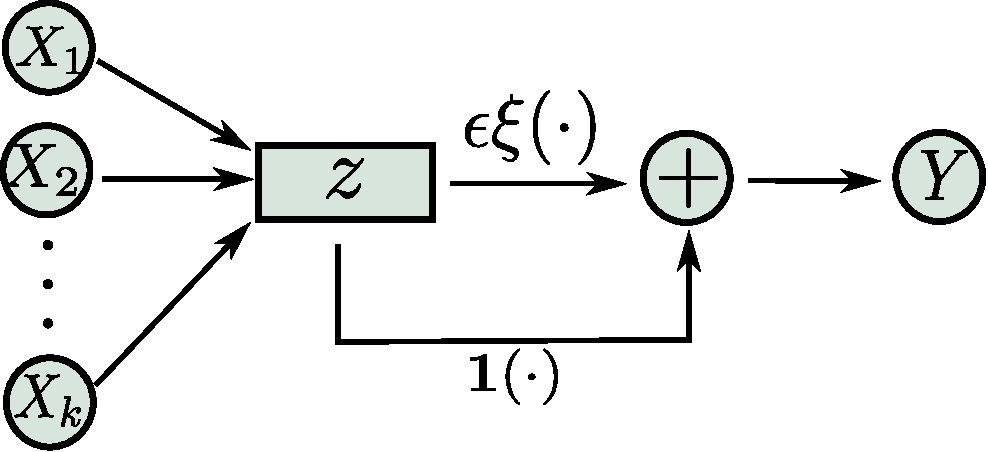
\includegraphics[width=\linewidth]{network_structure.pdf}
\caption{The structure of one-node neural network. The activation function $\sigma$ takes the form $\sigma(z)=z + \epsilon \xi(z)$.}
\label{fig:ns}
\end{figure}
\section{Related works}
Most existing theoretical works to explore the influnce of network structures focus on
the factor of layers and hidden units.
For example, \cite{kuri2017closed} determines the minimal number of hidden units for a multi-layered perceptron.
ReLU is used in \cite{AroraBMM18}, which focuses on studying the number of layers and hidden units.
We notice that these works are restricted on a specific activation function and seldom explore 
what is the best performance non-linear activation function can achieve for a certain network architecture.

To compensate this shortcoming, our study on activation function adopts the approach of statistical learning theory \cite{vapnik1999nature},
which samples the data from
a probablity distribution and finds a predictive function minimizing the expected value of the loss function.
Our theoretical result can explain previous empirical studies such as:
\begin{itemize}
\item Fixing the network structure, optimizing over parameterized activation function can improve the overall performance \cite{ramachandran2017searching}.
\item Using Hermite orthogonal polynomial as activation function works better than sigmoid
under certain conditions \cite{ma2005constructive}.
\end{itemize}

%%%%%%%%%%%%%%%%%%%%%%%%%%%%%%%%%%%%%%%%%%
\section{Mathematical Model}\label{sec:mm}
We consider one-node neural network, whose structure is shown in Figure \ref{fig:ns}.
Its input is a $k$-dimensional random vector $\underline{X}=(X_1, \dots, X_k)$ and it outputs a random variable $Y$.
Our goal is to predict $Y$ using $ \sigma(\sum_{i=1}^k w_i X_i)$.
For a given sampling result, we have $n$ data pairs $(\underline{x}_1, y_1), \dots, (\underline{x}_n, y_n)$, and
the $\ell_2$ loss function is given by
$\ell_2(\bm{x},\underline{y}) = \norm{\underline{y} - \sigma(\sum_{i=1}^k w_i \underline{x}_i)}^2 $
where $\underline{x}_i= (x_{1i}, \dots, x_{ni})^\T$ is the $i$-th column of the feature vector $\bm{x}$ and
$\underline{y} = (y_1, \dots, y_n)$ is the label vector. $\sigma$ is applied to a vector in elementwise way.
The optimal weight for a given activation function $\sigma$ is the minimizer of $\ell_2(\bm{x},\underline{y})$.

This type of network arises from function approximation problems, where a target function $g$, defined in a finite set,
is estimated by $\sigma(\sum_{i=1}^k w_i f_i)$. %and the domain of definition for $f_i, g$ is a finite set.
Suppose the ranges of $f_i, g$ are with cardinality $n$, 
then the functions themselves can be completely determined by $n$-dimensional vectors.
Furthermore, we assume each element from the ranges of $f_i, g$ is sampled from a distribution,
since we are considering the average performance over different $f_i, g$ pairs.
Then we can establish a correspondence between
$f_i$ and $\underline{x}_i$,
and between $g$ and $\underline{y}$.


In our model, we suppose $\bm{x},\underline{y}$ are drawn from
a joint distribution $G$.
That is, $\bm{x},\underline{y}$ are samples of random matrix $\bm{X}$ and random vector $\underline{Y}$.
We are interested to find a function $\sigma$ which minimizes
$\E[ \min_{\underline{w}} \ell_2(\bm{X},\underline{Y})]$.
Our requirement of the activation function $\sigma$ is that
$\sigma(z) = z + \epsilon \xi(z)$ where
$\epsilon$ is a small constant. The non-linear term should satisfy the normalization constraint
$\E[\xi(\bm{X}\underline{w})]=1$ where
$\bm{X}\underline{w} = \sum_{i=1}^k w_i \underline{X}_i$ is the matrix-vector product with  $\underline{w}=(w_1, \dots, w_k)$.

We formulate the universally optimal activation function $\sigma$ as follows:
\begin{Definition}\label{def:ug}
Let $(\bm{X}, \underline{Y})$ follow distribution $G$ and
$\mathcal{F}$ a function space for $\sigma(z)$. Then
we define the averaged estimation error $\mathrm{E}[\sigma]$ as
\begin{align}\label{eq:ug}
\mathrm{E}(\sigma) \triangleq & \E[ \min_{\underline{w}} \norm{\underline{Y} - \sigma(\bm{X} \underline{w})}^2] 
%s.t. \,& \sigma(z) = z + \epsilon \xi(z) \nonumber \\
%&\E[\norm{\xi(\bm{X}\underline{w})}^2]=1
\end{align}
The function $\sigma^*$ which minimizes $\mathrm{E}(\sigma)$
is called the universally optimal activation function for the one-node neural network,
i.e. $\sigma^* = \arg\min_{\sigma \in \mathcal{F}} \mathrm{E}(\sigma)$.
\end{Definition}

Definition \ref{def:ug} is a general formulation for any distribution space $G$.
To get analytical insights we should choose some specific distribution.
Therefore, in the following analysis, we assume:
\begin{enumerate}
\item $\underline{Y}$ follows Gaussian distribution $\mathcal{N}(\mathbf{0},\frac{1}{n} \mathbf{I}_n)$.
\item $\bm{X}$ is a $n\times k$ uniformly distributed random orthogonal matrix.
\item $\underline{Y}$ and $\bm{X}$ are independent.
\end{enumerate}
For assumption 2), the definition of uniformly distributed random orthogonal matrix is $\bm{X} \triangleq \bm{X}'(\bm{X}'^\T\bm{X}')^{-1/2}$
where elements of $\bm{X}'$ are i.i.d. $\mathcal{N}(0, 1)$ random variables \cite[Proposition 7.1]{eaton1989group}.
Since $\bm{X}^\T\bm{X} = \mathbf{I}_k$, $\bm{X}$ is indeed orthogonal matrix.
The definition of $\bm{X}$ can be regarded as the post-processing result of PCA (Principal Component Analysis)
on network input $\bm{X}'$ and weight $\underline{w}'$, because
we make the transformation $\bm{X} = \bm{X}'(\bm{X}'^\T\bm{X}')^{-1/2}, \underline{w} = (\bm{X}'^\T\bm{X}')^{1/2}\underline{w}'$.
We see that $\bm{X}'\underline{w}' = \bm{X}\underline{w}$.
%This completes the definition of the distribution space $G$.
%Such choice makes it possible for the analytical analysis of the averaged estimation error.
Based on the distribution space $G$ by 1)\,-3), for linear function space, we have the following conclusion:

\begin{Proposition}\label{prop:linear}
We have $\mathrm{E}(\sigma_0) = 1 - \frac{k}{n}$ where $\sigma_0(z) = z$ is the identity function.
\end{Proposition}

Proposition \ref{prop:linear} says that the averaged estimation error $\mathrm{E}$ for linear function is equal to $1-\frac{k}{n}$,
which is consistent with our intuition
since we use $k$ degrees of freedom to estimate arbitrary vector in $n$-dimensional space.



We have analyzed the averaged error for linear function.
To extend our result to non-linear functions, we need to choose a proper function space $\mathcal{F}$.
In this paper we consider a local region which contains non-linear function perturbed from the linear space.
The distance from non-linear function to linear space is quantified by a positive value $\epsilon$.
Thus we consider $\mathcal{F}_{\sigma_0}(\epsilon) =\{ \sigma \,|\, \norm{\sigma - \sigma_0} \leq \epsilon\}$.
Then all smooth functions can be treated as $\cup_{\epsilon>0} \mathcal{F}(\epsilon)$.
The norm of function is chosen as the expectation w.r.t. the distribution space $G$.
That is, $||\sigma - \sigma_0||^2\triangleq \E[\norm{(\sigma - \sigma_0)(\bm{A}\underline{Y})}^2] $
where $\bm{A} = \bm{X}\bm{X}^\T$.


We are particularly interested in how the averaged error changes
when $\sigma$ is contracted to $\sigma_0$ along a certain direction in $\mathcal{F}(\sigma)$.
That is, given a function $\xi$ we can construct $\sigma = \sigma_0 + \epsilon \xi$
where $\xi \in \mathcal{F}_0 = \{\xi | \norm{\xi} \leq 1 \}$. Then $\sigma \to \sigma_0$ is equivalent to $\epsilon \to 0$.

To measure the change rate of $E[\sigma]$ when $\sigma \to \sigma_0$,
we introduce the concept of the asymptotic error rate as follows:
\begin{Definition}
Let $\xi \in \mathcal{F}_0$, the asymptotic error rate for $\xi$ is
\begin{equation}\label{eq:Cxi}
\mathrm{C}[\xi] \triangleq \lim_{\substack{\epsilon \to 0 \\ \sigma = \sigma_0 + \epsilon \xi}} \frac{E[\sigma] - E[\sigma_0]}{\epsilon^2}
\end{equation}
\end{Definition}

$\mathrm{C}[\xi]$ can represent the error change rate of perturbation from linear function.
If $\mathrm{C}[\xi]$ is negative for a given $\xi$,
$\mathrm{E}[\sigma]$ decreases in the rate of $\abs{\mathrm{C}[\xi]}$ along the perturbation direction $\xi$,
which can be seen more clearly if we rewrite \eqref{eq:Cxi} as
$\mathrm{E}[\sigma] = \mathrm{E}[\sigma_0] +
\mathrm{C}[\xi]\epsilon^2 + o(\epsilon^2)$.
In this form, we can also see that $\mathrm{C}[\xi]$ is the coefficient of the second order term of $\mathrm{E}[\sigma]$.

To justify the definition of $\mathrm{C}[\xi]$, we need to show the limit in Equation \eqref{eq:Cxi} exists, which is guaranteed by the following proposition:
%For functional space $F$, we choose $P_m(z)$,
%which consists of polynomials with the highest degree no more than $m$.

\begin{Proposition}\label{prop:Esigma} 
Let $\nabla \xi(\underline{z})  = \diag[\xi'(\underline{z}_1), \dots, \xi'(\underline{z}_n)]$. Then we have
\begin{align}\notag
\mathrm{C}[\xi]= & \E[\norm{\xi(\bm{A}\underline{Y})}^2 -
\norm{\bm{X}^\T\xi(\bm{A}\underline{Y})}^2 \\
&- \norm{\bm{X}^\T \nabla\xi(\bm{A}\underline{Y})(Y-\bm{A}\underline{Y})}^2]
\end{align}
\end{Proposition}

Our goal is to get the fastest decreasing path $\xi$ from $E[\sigma_0]$ to $E[\sigma]$, this is equivalent to solve an optimization problem $\min \mathrm{C}[\xi]$ constraint by $\xi \in \mathcal{F}_0$.
It is hard to optimize $\xi$ over $\mathcal{F}_0$ directly, and we consider $\mathcal{F}_{0,m} = \mathcal{F}_0 \cap P_m$ instead. $P_m$ consists of polynomials with the degree no greater than $m$, and we have $\mathcal{F}_0 = \lim_{m\to \infty} \mathcal{F}_{0,m}$.

For $\xi \in \mathcal{F}_{0,m}$ we have the following result:
\begin{Proposition}\label{prop:quadratic}
If
$\xi(z) = \sum_{i=0}^m \underline{q}_i z^i$,
and $m \ll k$, then we have 
\begin{align}
\mathrm{C}[\xi] &= (1-\frac{k}{n}) \underline{p}^\T \mathbf{M} \underline{p} \notag\\
\textrm{where }\underline{p}_i &= \frac{k^{i/2}}{n^{- 1/2 + i}}\underline{q}_i\label{eq:pqt} \\
\mathbf{M}_{ij} =& -\ide{i}{j}(i-1)(j-1)(i+j-3)!! \notag
\end{align}
The constraint $\xi \in \mathcal{F}_{0,m}$ is equivalent with
\begin{align}
\underline{p}^\T \mathbf{N} \underline{p} & = 1 \textrm{ with }\notag\\
\mathbf{N}_{ij}  & = \ide{i}{j}(i+j-1)!!
\end{align}
\end{Proposition}

Proposition \ref{prop:quadratic} gives a feasible approach to choose the optimal $\xi$ by solving a quadratic optimization problem. We make the assumption $
m \ll k$ to write $M_{ij}$ in a concise form. This assumption requires that we should choose low degree polynomials as activation function and the number of node $k$ should be relatively large to represent features. Since computational cost
is proportional to the degree of polynomials and feature dimensions are usually high, our assumption does not lose practicality. 

\section{Hermite Polynomials}\label{sec:hp}

One of our major results is that we find Proposition \ref{prop:quadratic} leads naturally to the Hermite polynomials solutions.
(Probabilists') Hermite polynomials, denoted as $H_m(x),m=1,2,\dots$,
are defined as a series of polynomials satisfying the orthogonal property \linebreak$ \E[H_m(X)H_n(X)] = n! \mathrm{1}_{m=n}$ where $X$ is the standard normal random variable.
The degree of $H_m(x)$ is $m$.
Using Hermite polynomials, the minimizer of $\mathrm{C}[\xi]$ is expressed in the following way:
\begin{Proposition}\label{prop:value}
Let
\begin{equation}\label{eq:ximopt}
    \xi_m(z) \triangleq \frac{1}{\sqrt{m!n}} H_m\left(\frac{n}{k^{1/2}} z\right)
\end{equation}
Then $\mathrm{C}[\xi_m] = -(1-\frac{k}{n})(m-1) \leq \mathrm{C}[\xi] $ for all $\xi \in \mathcal{F}_{0,m}$.
\end{Proposition}
Proposition \ref{prop:value} also gives the expression of the minimal asymptotic error rate, which has linear relation with the degree of Hermite polynomials. This result is obtained
under the assumption $ m \ll k$. In general case when $ m \ll k$ does not hold, by numerical simulation we find that $-(1-\frac{k}{n})(m-1) < \mathrm{C}[\xi]$ while $\mathrm{C}[\xi]$ decreases in linear way.

\section{Experiment Result}\label{sec:er}

To verify the change rate of $C[\xi]$ is linear as we increase the maximal degree of polynomials $m$,
we conduct a simple experiment with $n=180, k=120$. We use $\xi_m(z)$ from Proposition
\ref{prop:value} and normalized polynomials with only the highest degree $\tilde{\xi}_m(z) = \frac{(nz/\sqrt{k})^m}{\sqrt{(2m-1)!!n}}$ as activation function. Using the Monte Carlo method to compute $\mathrm{C}[\xi]$ from Proposition \ref{prop:Esigma},
our experiment result is shown in Figure \ref{fig:fixednk}.
As can be seen, the Hermite polynomial results coincide with the theoretical lower bound in Proposition \ref{prop:value}.
For $\tilde{\xi}_m$, it cannot achieve the minimum value,
but we can still observe the nearly linear relationship between $C[\tilde{\xi}_m]$ and degree $m$.
From Equation \eqref{eq:pqt}, we also notice that for $\tilde{\xi}_m$,
the highest degree term contributes $-(1-\frac{k}{n})\frac{(m-1)^2}{2m-1}$ to $C[\xi]$,
which is approximately $\frac{1}{2} C[\xi_m]$.
This phenomenon suggests that the contribution of each polynomial
degree to $C[\xi]$ is not evenly distributed and
higher degree terms contribute more.  


\begin{figure}
    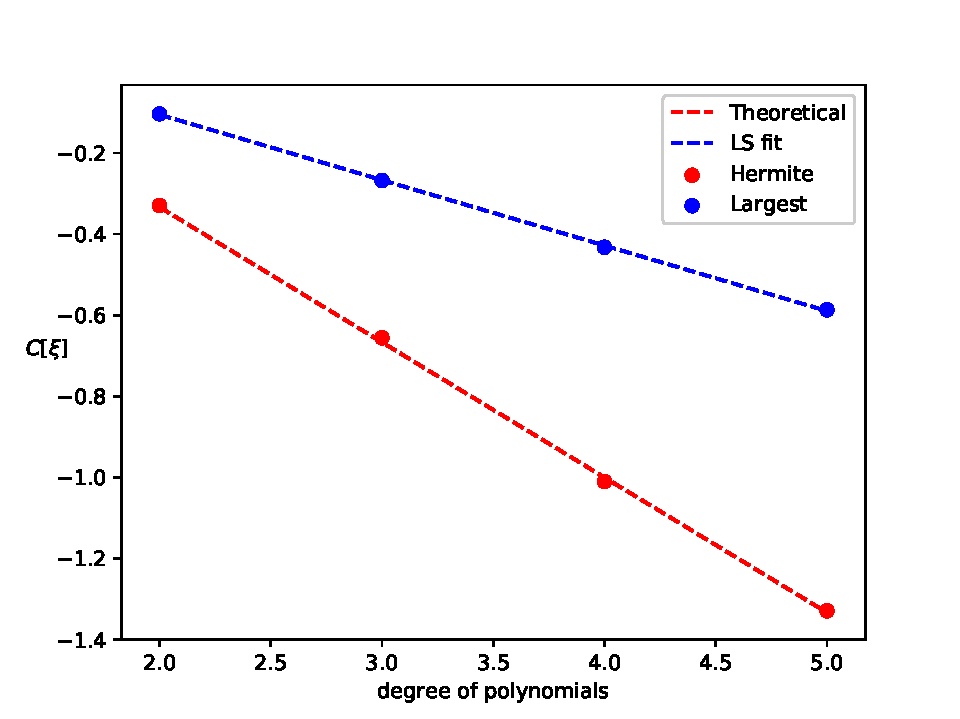
\includegraphics[width=\linewidth]{fixed_nk.pdf}
    \caption{Illustration of the linear decreasing property of $C[\xi]$.
    The dotted red line represents the theoretical lower bound $-(1-\frac{k}{m})(m-1)$
    while the dotted blue line is the least square fit of the empirical result by polynomials with only the highest degree.}\label{fig:fixednk}
\end{figure}


\section{Conclusion}\label{sec:con}

In this paper, we have investigated the mechanism of non-linearity in one-node neural network.
If we add polynomial perturbation to linear activation function,
the network loss is linearly decreased as the degree of polynomial is increased. How non-linearity works in more complex neural networks will be considered in the future. 

%\section{Proofs}
%%%%%%%%%%%%%%%%%%%%%%%%%%%%%%%%%%%%%%%%%%
\vspace{6pt} 

%%%%%%%%%%%%%%%%%%%%%%%%%%%%%%%%%%%%%%%%%%
%% optional
%\supplementary{The following supporting information can be downloaded at:  \linksupplementary{s1}, Figure S1: title; Table S1: title; Video S1: title.}

% Only for the journal Methods and Protocols:
% If you wish to submit a video article, please do so with any other supplementary material.
% \supplementary{The following supporting information can be downloaded at: \linksupplementary{s1}, Figure S1: title; Table S1: title; Video S1: title. A supporting video article is available at doi: link.}

%%%%%%%%%%%%%%%%%%%%%%%%%%%%%%%%%%%%%%%%%%
\authorcontributions{Methodology, validation, formal analysis, writing---original draft preparation: Feng Zhao; Conceptualization,  writing---review and editing, supervision, project administration, funding acquisition:
Shao-Lun Huang. All authors have read and agreed to the published version of the manuscript.}

\funding{This research was funded in part by the Shenzhen Science and Technology Program under Grant KQTD20170810150821146, National Key R\&D Program of China under Grant 2021YFA0715202 and High-end Foreign Expert Talent Introduction Plan under Grant G2021032013L.}

\institutionalreview{Not applicable}

\informedconsent{Not applicable}

\dataavailability{Not applicable} 

%\acknowledgments{}

\conflictsofinterest{The authors declare no conflict of interest.} 

%%%%%%%%%%%%%%%%%%%%%%%%%%%%%%%%%%%%%%%%%%
%% Optional
%\sampleavailability{Samples of the compounds ... are available from the authors.}

%% Only for journal Encyclopedia
%\entrylink{The Link to this entry published on the encyclopedia platform.}

\abbreviations{Abbreviations}{
The following abbreviations are used in this manuscript:\\

\noindent 
\begin{tabular}{@{}ll}
MMSE & Minimum Mean Square Error \\
ResNets & Residual Neural Networks\\
PCA & Principal Component Analysis\\
\end{tabular}
}

%%%%%%%%%%%%%%%%%%%%%%%%%%%%%%%%%%%%%%%%%%
%% Optional
\appendixtitles{no} % Leave argument "no" if all appendix headings stay EMPTY (then no dot is printed after "Appendix A"). If the appendix sections contain a heading then change the argument to "yes".
\appendixstart
\appendix
\section[\appendixname~\thesection]{Proofs}\label{sec:Proofs}
\begin{Lemma}\label{lem:A}
	Suppose $\bm{X}$ is a uniformly distributed random orthogonal matrix and $\bm{A} = \bm{X}\bm{X}^\T$,
	then $\E[\bm{A}] = \frac{k}{n} \mathbf{I}_n$.
\end{Lemma}
\begin{proof}[Proof of Lemma \ref{lem:A} ]
By the symmetric property we only need to show $\E[\bm{A}_{11}] = \frac{k}{n}$ and
$\E[\bm{A}_{12}] = 0$. For the first equation, we have $n\E[\bm{A}_{11}]
= \sum_{i=1}^n \E[\bm{A}_{ii}] = \sum_{i=1}^n \E[ \sum_{j=1}^k \bm{X}^2_{ij}] =
\sum_{j=1}^k \E[\sum_{i=1}^n \bm{X}^2_{ij}]$. Since the norm of $\bm{X}_j$ is 1,
the whole summation evaluates to $k$. Therefore $\E[\bm{A}_{11}] = \frac{k}{n}$.

On the other hand, $\bm{X}$ can be treated as an $n\times k$ subblock of an $n\times n$
random orthogonal matrix $\bm{\bar{X}}$ with the property that $\bm{X}_{ij} = \bm{\bar{X}}_{ij}$
for $j\leq k$. For $\bm{\bar{X}}$, the first and second row are orthogonal:
 $\E[\sum_{j=1}^n \bm{\bar{X}}_{1j}\bm{\bar{X}}_{2j}] = 0 $ which leads to
 $\E[\bm{X}_{1j}\bm{X}_{2j}] = 0$ for $j \leq k$. Hence $\E[\bm{A}_{12}]=
 \E[\sum_{j=1}^k \bm{X}_{1j}\bm{X}_{2j}]=0$.
\end{proof}
\begin{proof}[Proof of Proposition \ref{prop:linear}]
    When $\epsilon = 0$, the optimal $\underline{w}_0 = \bm{X}^\T\underline{Y}$. Therefore
    $\E[\norm{\underline{Y} - \sigma(\bm{X} \underline{w}_0)}^2] = \E[\norm{\underline{Y}-\bm{X}\bm{X}^\T\underline{Y}}^2]$.
    The expectation can be taken by $\underline{Y}$ first and then by $\bm{X}$.
    Let $\underline{Z} = (I-\bm{A}) \underline{Y}$, and $Z$ is a Gaussian random vector
    for given $\bm{X}$. Therefore, $\E_{\underline{Y}}[\norm{\underline{Z}}^2] = \Tr[(I-A)^\T\Cov[Y](I-A)]
    = \frac{1}{n}\Tr[I - A]$. Using Lemma \ref{lem:A}, $\mathrm{E}(\sigma) = 1 - \frac{k}{n}$ follows.
\end{proof}
\begin{proof}[Proof of Proposition \ref{prop:Esigma} ]
For the problem $\min_{\underline{w}} \norm{\underline{Y} - \sigma(\bm{X} \underline{w})}$
with $\sigma = \sigma_0 + \epsilon \xi$. We can write $\underline{w} = \underline{w}_0
+ \epsilon \underline{\hat{w}} + o(\epsilon)$ where $\underline{w}_0 = \bm{X}^\T \underline{Y}$ is the minimizer for
$\epsilon = 0$. That is, we assume $\underline{w}$ can be expanded near $\underline{w}_0$
using $\epsilon$ terms. We can expand $\norm{\underline{Y} - \sigma(\bm{X} \underline{w})}$ 
up to $o(\epsilon^2)$ as
\begin{align*}
&\norm{\underline{Y} - \bm{X} \underline{w}_0 - \epsilon \bm{X} \underline{\hat{w}} -
\epsilon^2 \bm{X} \underline{\tilde{w}} - \epsilon \xi(\bm{X} \underline{w}_0 +
\epsilon \bm{X} \underline{\hat{w}}) }^2 \\
&\quad=  \norm{ \underline{Y} - \bm{X}  \underline{w}_0 -
\epsilon (\bm{X}\underline{\hat{w}} + \xi(\bm{X} \underline{w}_0 )) \\
&\qquad-  \epsilon^2(\bm{X}\underline{\tilde{w}} + \nabla \xi(\bm{X} \underline{w}_0 )\bm{X}\underline{\hat{w}})}^2 \\
&\quad=  \norm{\underline{Y}-\bm{X} \underline{w}_0  }^2 -
2 \epsilon (\bm{X} \underline{\hat{w}} +
\xi(\bm{X} \underline{w}_0))^\T (\underline{Y} - \bm{X} \underline{w}_0) \\
& \qquad+  \epsilon^2(\norm{\bm{X}\underline{\hat{w}} + \xi(\bm{X} \underline{w}_0)}^2 \\
& \qquad\quad -
2 (\bm{X} \underline{\tilde{w}}+
\nabla \xi(\bm{X} \underline{w}_0)\bm{X}\underline{\hat{w}})^\T(\underline{Y}-\bm{X} \underline{w}_0))
\end{align*}
$\bm{X}\underline{w}_0 = \bm{X}\bm{X}^\T \underline{Y}$ is the projection of $\underline{Y}$ onto linear subspace spanned by
columns of $\bm{X}$.

We first show that in the expansion of $\E[\sigma]$, the coefficient of $\epsilon$-term is zero.
We define $\tilde{\underline{Y}} = -\underline{Y} + 2\bm{X}\bm{X}^T\underline{Y}$, which is
the mirror of $\underline{Y}$ about linear subspace spanned by $\bm{X}\bm{X}^T$.
Then we have
$\bm{X}\bm{X}^\T \underline{Y} = \bm{X}\bm{X}^\T \tilde{\underline{Y}}$ and
$(\underline{Y}- \bm{X}\bm{X}^\T\underline{Y}) = -(\tilde{\underline{Y}} - \bm{X}\bm{X}^\T \tilde{\underline{Y}})$.
The density function $p_{\underline{Y}}$ satisfies $p_{\underline{Y}}(\underline{Y})=p_{\underline{Y}}(\tilde{\underline{Y}})$.
These symmetric properties lead to $\E_{\underline{Y}}[\xi(\bm{X}\underline{w}_0)^\T (\underline{Y}-\bm{X}\underline{w}_0)]=0$.
On the other hand, since $\bm{X}^\T \bm{X} = \mathbf{I}_k$,
we have
$(\bm{X}\underline{\hat{w}})^\T (\underline{Y}-\bm{X}\underline{w}_0) = \underline{\hat{w}}^\T (X^\T \underline{Y} - \underline{w}_0) = 0$.

Next, we minimize the coefficient of $\epsilon^2$ by $\underline{\hat{w}}$, which is simplified to 
\begin{equation}\label{eq:st}
\norm{\bm{X}\underline{\hat{w}} + \xi(\bm{X} \underline{w}_0)}^2-
2 (
\nabla \xi(\bm{X} \underline{w}_0)\bm{X}\underline{\hat{w}})^\T(\underline{Y}-\bm{X} \underline{w}_0)
\end{equation}
due to $(\bm{X}\underline{\tilde{w}})^\T (\underline{Y}-\bm{X}\underline{w}_0) = 0 $.
The expression in \eqref{eq:st} is quadratic about $\underline{\hat{w}}$. The minimum value is achieved  at
$$
\underline{\hat{w}} =  \bm{X}^\T(\nabla\xi(\bm{X}\bm{X}^\T \underline{Y})
(\underline{Y}-\bm{X}\bm{X}^\T \underline{Y}) - \xi(\bm{X}\bm{X}^\T \underline{Y}))
$$
Substituting $\underline{\hat{w}}$ in expression in \eqref{eq:st} with the above equation we can get the minimum value for the coefficient of $\epsilon^2$, which is exactly $C[\xi]$.
%\begin{align*}
%C[\xi] = & \E[\norm{\xi(\bm{X}\bm{X}^\T\underline{Y})}^2 -
%\norm{\bm{X}^\T\xi(\bm{X}\bm{X}^\T\underline{Y})}^2 \\
%& -
%\norm{\bm{X}^\T \nabla\xi(\bm{X}\bm{X}^\T\underline{Y})(\underline{Y}-\bm{X}\bm{X}^\T\underline{Y})}^2]
%\end{align*}
\end{proof}
\begin{Lemma}\label{lemma:Isserlis2}
     Suppose $(X,Y)$ follows two-dimensional Gaussian distribution $\mathcal{N}(\bm{0}, \Sigma)$, then for the case $i+j$ is even, we have
\begin{equation*}
    \E[X^i Y^j] =
    \sum_{k=0}^{\min\{i,j\}}
    \frac{\ide{k}{i} i! j!}{k! (i-k)!!(j-k)!!}
    \Sigma_{12}^k \Sigma_{11}^{(i-k)/2}\Sigma_{22}^{(j-k)/2}
\end{equation*}
\end{Lemma}
\begin{proof}
Using Isserlis' theorem \cite{isserlis1918formula} we obtain
$  \E[X^i Y^j] = \sum_{k=0}^{\min\{i,j\}} C_k \Sigma_{12}^k \Sigma_{11}^{(i-k)/2}\Sigma_{22}^{(j-k)/2}$.
The power of $\Sigma_{11}$ should be an integer. Therefore, if $\ide{k}{i} = 0$, $C_k = 0$.
For $\ide{k}{i} = 1$, we choose $k$ items of $X$ and $Y$ to form $\Sigma_{12} = \E[XY]$, which has $\binom{i}{k}\binom{j}{k}$ choices.
For the remaining $(i-k)$ numbers of $X$, we should pair them. There are $\frac{1}{(\frac{i-k}{2})!}\prod_{i=1}^{(i-k)/2} \binom{2i}{2} = \frac{(i-k)!}{(i-k)!!}$ possible combinations; For $(j-k)$ numbers of $Y$, it is $\frac{(j-k)!}{(j-k)!!}$; Finally, for $k$ pairs of $XY$, there are $k!$ possible combinations. The product $\binom{i}{k}\binom{j}{k}\frac{(i-k)!}{(i-k)!!}\frac{(j-k)!}{(j-k)!!}k!$ is the coefficient $C_k$.
\end{proof}
%\begin{lemma}\label{lemma:A1112}
%For random matrix $\bm{A}$ we have $\E[\bm{A}_{11}^t] = \prod_{i=0}^{t-1} \frac{k+2t}{n+2t}$ and
%$\E[\bm{A}_{12}^2] = \frac{(n-k)k}{(n-1)n(n+2)}$.
%\end{lemma}
%\begin{proof}[Proof of Lemma \ref{lemma:A1112}]
%Then the high order moment of $\bm{A}_{11}^t$ follows from \cite[Eq. 8]{weisstein}. To compute $\E[\bm{A}_{12}^2]$, using the symmetric property first we %have $\E[\bm{A}_{11}^2] = k\E[\bm{X}_{11}^4] + k(k-1)\E[\bm{X}_{11}^2 \bm{X}_{12}^2] \Rightarrow
%\frac{k(k+2)}{n(n+2)} = \frac{3k}{n(n+2)} + (k-1) (k \E[\bm{X}_{11}^2 \bm{X}_{12}^2])$.
%Also $\E[\bm{A}_{12}^2] = \E[(\sum_{i=1}^k \bm{X}_{11} \bm{X}_{12})^2]
%= k \E[\bm{X}_{11}^2\bm{X}_{12}^2] + k(k-1)\E[\bm{X}_{11}\bm{X}_{12}\bm{X}_{21}\bm{X}_{22}]
%$.
%Since $\sum_{i=1}^n \bm{X}_{1i} \bm{X}_{2i} = 0$, multiplying this equation by $\bm{X}_{12}\bm{X}_{22}$ and taking the expectation
%we have $\E[\bm{X}_{11}\bm{X}_{12}\bm{X}_{21}\bm{X}_{22}] = \frac{-1}{n-1} \E[\bm{X}^2_{11}\bm{X}^2_{12}]$.

%Therefore $\E[\bm{A}^2_{12}]=(1-\frac{k-1}{n-1}) \frac{k}{n(n+2)}$.
%\end{proof}
\begin{Lemma}\label{lemma:UUN}
    \begin{align}
        &\ide{i}{j} (i+j-1)!! = \sum_{k=0}^{\min\{i, j\}}
        \ide{k}{i} \ide{k}{j} \frac{i! j!}{(i-k)!!(j-k)!! k!} \label{eq:UUN} \\
             &   \ide{i}{j}(i-1)(j-1)(i+j-3)!!  \notag\\
        &=\sum_{k=0}^{\min\{i, j\}}
        \ide{k}{i} \ide{k}{j} \frac{(k-1)i!j!}{(i-k)!!(j-k)!!k!} \label{eq:UUM}
    \end{align}
\end{Lemma}
\begin{proof}[Proof of Lemma \ref{lemma:UUN} ]
	If $ i + j $ is odd, $ \ide{i}{j} = 0 $ and
	$ \ide{k}{i}\ide{k}{j} = 0 $. Then Equation \eqref{eq:UUN} holds.
	Therefore, we only need to consider the case if $ i + j $ is even.
	First we define $A(i, j) = \sum_{k=0}^{\min\{i, j\}}
	\ide{k}{i} \ide{k}{j} \frac{i! j!}{(i-k)!!(j-k)!! k!}$.
	Then we can show that
	\begin{align*}
	& A(2i+1, 2j+1) = (2i + 1) A(2i, 2j) + (2j) A(2i+1, 2j-1)\\
	& A(2i, 2j)= (2j - 1) A(2i, 2j-2) + (2i) A(2i-1, 2j-1) 
	\end{align*}
	Then using mathematical induction we have $A(i,j) = (i+j-1)!!$ if $i + j $ is even.
	Based on our discussion on the parity of $i+j$, in general we have $A(i,j)=\ide{i}{j}(i+j-1)!!$.
	Equation \eqref{eq:UUM} follows by applying \eqref{eq:UUN}.
\end{proof}

\begin{proof}[Proof of Proposition \ref{prop:quadratic}]
Let $\underline{Z} = \bm{A}\underline{Y}, \underline{Z}' = (\mathbf{I} - \bm{A})\underline{Y}$. Given $\bm{X}$, $\underline{Z}$ is Gaussian vector with covariance matrix $\bm{A} \Cov[\underline{Y}] \bm{A}^\T = \frac{\bm{A}}{n}$. Similarly, $\Cov[\underline{Z}'] = \frac{\mathbf{I} - \bm{A}}{n}$. Using $\bm{A}^2 = \bm{A}$ we have $\E[\underline{Z}'\underline{Z}^\T] = 0$. That is, $\underline{Z}'$ and $\underline{Z}$ are independent, and we have $\E[f(\underline{Z}_i)g(\underline{Z}'_j)] = \E[f(\underline{Z}_i)]\E[g(\underline{Z}'_j)]$ for arbitrary function.
    
Let $\mathrm{C}_1 = \E_{\underline{Y}} [\norm{\xi(\bm{A}\underline{Y})}^2]$, $\mathrm{C}_2 
= \E_{\underline{Y}}
[\norm{\bm{X}^\T\xi(\bm{A}\underline{Y})}^2]$, $\mathrm{C}_3 
= \E_{\underline{Y}}
[\norm{\bm{X}^\T \nabla\xi(\bm{A}\underline{Y})(\underline{Y}-\bm{A}\underline{Y})}^2]$,
$\mathrm{C}[\bm{X}, \xi] :=  \mathrm{C}_1 - \mathrm{C}_2 - \mathrm{C}_3$. Then $\mathrm{C}[\xi] = \E_{\bm{X}}[\mathrm{C}[\bm{X}, \xi]]$,
and we have
\begin{align*}
    \mathrm{C}_1 &=\E[\norm{\xi(\underline{Z})}^2] = \sum_{i=1}^n \E[\xi^2(\underline{Z}_i)] \\
    \mathrm{C}_2 &= \sum_{i,j=1, i \neq j}^n \bm{\bm{A}}_{ij}\E[\xi(\underline{Z}_i)\xi(\underline{Z}_j)] +
    \sum_{i=1}^n \bm{\bm{A}}_{ii}  \E[\xi^2(\underline{Z}_i)]\\
    \mathrm{C}_3 & = \sum_{i,j=1, i \neq j}^n \bm{A}_{ij}\bm{\Sigma}_{ij} +
    \sum_{i=1}^n \bm{A}_{ii}\bm{\Sigma}_{ii}     \textrm{ where }\\
    \bm{\Sigma}_{ii} &=  \E[ [\underline{Z}'_i]^2 [\xi'(\underline{Z}_i)]^2] = \frac{1-\bm{A}_{ii}}{n}\E[\xi'^2(\underline{Z}_i)]   \\
    \bm{\Sigma}_{ij} &=  \E[\underline{Z}'_i \underline{Z}'_j \xi'(\underline{Z}_i)
    \xi'(\underline{Z}_j)]
     =  \frac{-\bm{A}_{ij}}{n} \E[ \xi'(\underline{Z}_i)
    \xi'(\underline{Z}_j)]
\end{align*}
%The expression for $\Sigma_{ij}$ holds for $i \neq j$ above.
Combining the above equations we have
\begin{align*}
   &  \mathrm{C}[\bm{X}, \xi] = \sum_{i=1}^n (1-\bm{A}_{ii})(\E[\xi^2(\underline{Z}_i)] -
    \frac{ \bm{A}_{ii}}{n} \E[ \xi'^2(\underline{Z}_i)]) \\
    &- \sum_{i,j=1, i \neq j}^n \bm{A}_{ij} (\E[\xi(\underline{Z}_i)\xi(\underline{Z}_j)] -
    \frac{\bm{A}_{ij}}{n}\E[\xi'(\underline{Z}_i) \xi'(\underline{Z}_j)])
\end{align*}
The summation term contributes equally to $\E_{\bm{X}}[\mathrm{C}[\bm{X}, \xi]]$. Therefore, will a little abuse of notation,
we can rewrite $\mathrm{C}[\bm{X}, \xi]$ as:
\begin{align*}
    &  \mathrm{C}[\bm{X}, \xi] =n(1-\bm{A}_{11})(\E[\xi^2(\underline{Z}_1)] -
    \frac{\bm{A}_{11}}{n}  \E[ \xi'^2(\underline{Z}_1)]) \\
    &- n(n-1)\bm{A}_{12}(\E[\xi(\underline{Z}_1)\xi(\underline{Z}_2)] -
    \frac{\bm{A}_{12}}{n}\E[\xi'(\underline{Z}_1)
   \xi'(\underline{Z}_2)])\nonumber
\end{align*}

Since 
$\xi(z) = \sum_{i=0}^m \underline{q}_i z^i $, we can rewrite $\mathrm{C}[\bm{X}, \xi]$
as the quadratic form $ \underline{q}^T \bm{M} \underline{q} $.
where $\bm{M}$ is an $(m+1) \times (m+1) $ random matrix 
whose element $\bm{M}_{ij}$ is given by
\begin{align*}
    \bm{M}_{ij} &= n(1-\bm{A}_{11}) (\E[\underline{Z}_1^{i+j}] -
    ij \frac{1}{n}\bm{A}_{11} \E[\underline{Z}_1^{i+j-2}])  \\
    &\quad -n(n-1)\bm{A}_{12}(\E[\underline{Z}_1^i \underline{Z}_2^j] - ij \frac{1}{n}\bm{A}_{12}\E[\underline{Z}_1^{i-1}\underline{Z}_2^{j-1}])
\end{align*}
Since $\bm{Z}_1$ is Gaussian, we have $\E[Z_1^{2t}] = \frac{1}{n^t}\bm{A}_{11}^t (2t-1)!!$. If $\ide{i}{j} = 0$, then $\bm{M}_{ij}=0$. Otherwise,
let $ 2t = i + j $, from Lemma \ref{lemma:Isserlis2}, $\E[\underline{Z}_1^i \underline{Z}_2^j]$ can be expanded, and we have:
\begin{align*}
    &\bm{M}_{ij} = -n(1-\bm{A}_{11}) \frac{\bm{A}_{11}^t}{n^t}(i-1)(j-1)(2t-3)!! \\
    &-\frac{n(n-1)\bm{A}_{12}}{n^t}\sum_{s=0}^{\min\{i,j\}}
    \frac{\ide{s}{i}(1-s)i!j!}{s!(i-s)!!(j-s)!!}
    \bm{A}_{12}^s \bm{A}_{11}^{\frac{i - s}{2}}\bm{A}_{22}^{\frac{j - s}{2}}
\end{align*}
$C[\xi] = \E_{\bm{X}}[\mathrm{C}[\bm{X}, \xi]] =  \underline{q}^T \mathbf{M}' \underline{q}$
where $\mathbf{M}'_{ij} = \E_{\bm{X}} [\bm{M}_{ij}] = -M_1 + M_2$
and 
\begin{align*}
    M_1 & =   \frac{\E[\bm{A}_{11}^t]-\E[\bm{A}_{11}^{t+1}]}{n^{t-1}}(i-1)(j-1)(2t-3)!! \\
    M_2 & = \frac{n-1}{n^{t-1}}\sum_{s=0}^{\min\{i,j\}}
    \frac{\ide{s}{i}(s-1)i!j!}{s!(i-s)!!(j-s)!!}
    \E[\bm{A}_{12}^{s+1} \bm{A}_{11}^{\frac{i - s}{2}}\bm{A}_{22}^{\frac{j - s}{2}}]
\end{align*}
Below we consider the case when $k, n \to +\infty$ while $m$ is finite. Since $\bm{A}=\bm{X}\bm{X}^\T$, from Proposition 7.2 of \cite{eaton1989group} we can get $\bm{A}_{11}$ is Beta distribution with parameter $B(\frac{k}{2}, \frac{n-k}{2})$.
From Theorem 1 of \cite{multivariateBeta},
$\E[\bm{A}_{11}^t]-\E[\bm{A}_{11}^{t+1}] = (1-r)\prod_{s=0}^{t-1} \frac{2s+k}{2s+n+2} \sim (1-r)r^t$ where
$ r \triangleq \frac{k}{n}$. Therefore, $M_1 \sim \frac{(1-r)r^t}{n^{t-1}}(i-1)(j-1)(2t-3)!!$.
We consider the case when $s+1$ is even, $\E[\bm{A}_{12}^{s+1} \bm{A}_{11}^{\frac{i - s}{2}}\bm{A}_{22}^{\frac{j - s}{2}}] \leq \sqrt{\E[\bm{A}_{12}^{s+1}\bm{A}_{11}^{i-s}]\E[\bm{A}_{12}^{s+1}\bm{A}_{22}^{j-s}]}$. When $k, n$ are sufficiently large, we can treat $\bm{A}_{11}, \bm{A}_{12}$ as joint Gaussian. From Theorem 2 of \cite{multivariateBeta}: $\E[\bm{A}_{12}^{s+1}\bm{A}_{11}^{i-s}] \sim s!! r^{i-s}(\frac{r(1-r)}{n})^{(s+1)/2}$. Similarly, $\E[\bm{A}_{12}^{s+1}\bm{A}_{22}^{j-s}] \sim s!! r^{j-s}(\frac{r(1-r)}{n})^{(s+1)/2}$. It implies that $\E[\bm{A}_{12}^{s+1} \bm{A}_{11}^{\frac{i - s}{2}}\bm{A}_{22}^{\frac{j - s}{2}}] \leq (s!!) r^{t-s}(\frac{r(1-r)}{n})^{(s+1)/2}$. We can get an upper bound of $M_2$ using Equation \ref{eq:UUM}: $M_2 \leq \frac{1}{n^{t-2}} (i-1)(j-1)(2t-3)!!\E[\bm{A}_{12}^{4} \bm{A}_{11}^{\frac{i - 3}{2}}\bm{A}_{22}^{\frac{j - 3}{2}}] \leq \frac{(1-r)^2 r^{t-1}}{n^t}3(i-1)(j-1)(2t-3)!!= \frac{3(1-r)}{k} M_1$.
When $k \to \infty$, we see that $M_2$ can be ignored and $\mathbf{M}'_{ij} = -\ide{i}{j}\frac{(1-r)r^t}{n^{t-1}}(i-1)(j-1)(2t-3)!!$. By changing of variables in Equation \ref{eq:pqt} we can get the correspondence $\mathbf{M}_{ij} = \frac{n^{-1+2t}}{k^t} \mathbf{M}'_{ij} = -\ide{i}{j}(1-r)(i-1)(j-1)(2t-3)!!$. 

To get the constraint on $\underline{q}$, we should choose $\norm{\xi} = 1$, which is equivalent to $\E_{\bm{X}}[\mathrm{C}_1] = 1$. By some computation we can get the expression of $\mathrm{N}$ when $ m \ll k$.

\end{proof}

\begin{Lemma}\label{lemma:Upem}
Let $\mathbf{U}$ be an $(m+1) \times (m+1)$ upper triangular matrix defined by\linebreak
$U_{ij} = \ide{i}{j} \frac{j!}{(j-i)!!\sqrt{i!}} \textrm{ for } 0 \leq i\leq j \leq m$, $\underline{e}_m$ is an $(m+1)$ dimensional vector whose elements are zero except that the last element is 1. $\underline{p}_i = \ide{i}{m} (-1)^{(m-i)/2}\frac{\sqrt{m!}}{i!(m-i)!!}$.
Then we have $ \mathbf{U} \underline{p} = \underline{e}_m$.
\end{Lemma}
\begin{proof}[Proof of Lemma \ref{lemma:Upem} ]
    For $ i = m, \mathbf{U}_{mm} = \sqrt{m!}$, and we can show that $\mathbf{U}_{mm} \underline{p}_m = 1 $; For $ 0\leq i < m $ we
    will show that $ \sum_{j=i}^m \mathbf{U}_{ij} \underline{p}_j = 0 $. In specific form as
    \begin{equation}\label{eq:jimf}
    \sum_{j=i}^m \ide{i}{j} \frac{j!}{(j-i)!!\sqrt{i!}}  \frac{\ide{j}{m}(-1)^{(m-j)/2}\sqrt{m!}}{j!(m-j)!!} = 0
    \end{equation}
    If $ \ide{i}{m} = 0$, $\ide{i}{j}\ide{j}{m} = 0$ and Equation \eqref{eq:jimf} holds. Otherwise, let $2m' = m - i$,    
    and Equation \eqref{eq:jimf} is equivalent to
    $ \sum_{j=i, \ide{i}{j}=1}^m  \frac{(-1)^{(m-j)/2}}{(m-j)!!(j-i)!!}  = 0  \iff  $
    $\sum_{j=0, j \textrm{ is even}}^{2m'}  \frac{(-1)^{(2m'-j)/2}}{(2m'-j)!! j!!}= 0  \iff $
    $\sum_{j=0}^{m'}  \frac{(-1)^{m'-j}}{(2m'-2j)!! (2j)!!} = 0  \iff $
    $\sum_{j=0}^{m'}  \frac{(-1)^{m'-j}}{(m'-j)! j!} = 0  \iff \sum_{j=0}^{m'} (-1)^{m'-j} \binom{m'}{j} = 0$
    $ \iff (1+x)^{m'} = 0 \,(x=-1)$.
\end{proof}
\begin{proof}[Proof of Proposition \ref{prop:value} ]
    Let $\mathbf{U}$ be the same matrix defined in Lemma \ref{lemma:Upem}. From Lemma \ref{lemma:UUN} we have $\mathbf{N}_{ij} = \sum_{k=0}^m \mathbf{U}_{ki}\mathbf{U}_{kj}$. Therefore, $\mathbf{N} = \mathbf{U}^\T\mathbf{U}$. Let $\Lambda = \diag[1, 0, -1, \dots, 1-m]$, from Equation \ref{eq:UUM} we have $\mathbf{M}_{ij} = \sum_{k=0}^m \mathbf{U}_{ki}\Lambda_{kk}\mathbf{U}_{kj}$. Therefore, $\mathbf{M} = \mathbf{U}^\T\Lambda\mathbf{U}$. Then $\min_{\underline{p}^\T N \underline{p} = 1} \underline{p}^\T \mathbf{M}\underline{p} = \min_{\underline{\tilde{p}}^\T\underline{\tilde{p}} = 1} \sum_{k=0}^m (1-k)\underline{\tilde{p}}_k^2 = 1-m$. We have made the invertible transformations $\underline{\tilde{p}} = \mathbf{U}\underline{p}$. Since the minimum value is achieved at $\underline{\tilde{p}} = \underline{e}_m$, from Lemma \ref{lemma:Upem} we have $\underline{p}_i = \ide{i}{m} (-1)^{(m-i)/2}\frac{\sqrt{m!}}{i!(m-i)!!}$. Equation \eqref{eq:ximopt} follows by transforming $\underline{p}$ back to $\underline{q}$ using Equation \eqref{eq:pqt} and comparing the expression of $\underline{q}$ with the explicit formula of probabilists' Hermite polynomials \cite[Eq. 18.5.13]{NIST:DLMF}.
\end{proof}
%%%%%%%%%%%%%%%%%%%%%%%%%%%%%%%%%%%%%%%%%%
\begin{adjustwidth}{-\extralength}{0cm}
%\printendnotes[custom] % Un-comment to print a list of endnotes

\reftitle{References}

% Please provide either the correct journal abbreviation (e.g. according to the “List of Title Word Abbreviations” http://www.issn.org/services/online-services/access-to-the-ltwa/) or the full name of the journal.
% Citations and References in Supplementary files are permitted provided that they also appear in the reference list here. 

%=====================================
% References, variant A: external bibliography
%=====================================
\bibliography{exportlist.bib}

%=====================================
% References, variant B: internal bibliography
%=====================================

% If authors have biography, please use the format below
%\section*{Short Biography of Authors}
%\bio
%{\raisebox{-0.35cm}{\includegraphics[width=3.5cm,height=5.3cm,clip,keepaspectratio]{Definitions/author1.pdf}}}
%{\textbf{Firstname Lastname} Biography of first author}
%
%\bio
%{\raisebox{-0.35cm}{\includegraphics[width=3.5cm,height=5.3cm,clip,keepaspectratio]{Definitions/author2.jpg}}}
%{\textbf{Firstname Lastname} Biography of second author}

% For the MDPI journals use author-date citation, please follow the formatting guidelines on http://www.mdpi.com/authors/references
% To cite two works by the same author: \citeauthor{ref-journal-1a} (\citeyear{ref-journal-1a}, \citeyear{ref-journal-1b}). This produces: Whittaker (1967, 1975)
% To cite two works by the same author with specific pages: \citeauthor{ref-journal-3a} (\citeyear{ref-journal-3a}, p. 328; \citeyear{ref-journal-3b}, p.475). This produces: Wong (1999, p. 328; 2000, p. 475)

%%%%%%%%%%%%%%%%%%%%%%%%%%%%%%%%%%%%%%%%%%
%% for journal Sci
%\reviewreports{\\
%Reviewer 1 comments and authors’ response\\
%Reviewer 2 comments and authors’ response\\
%Reviewer 3 comments and authors’ response
%}
%%%%%%%%%%%%%%%%%%%%%%%%%%%%%%%%%%%%%%%%%%
\end{adjustwidth}
\end{document}

